\documentclass[Thesis.tex]{subfiles}
\begin{document}

\chapter{{\sc ConformalLab} - Conformal maps and uniformization}
\label{chp:conformallab}

\begin{figure}
\centering
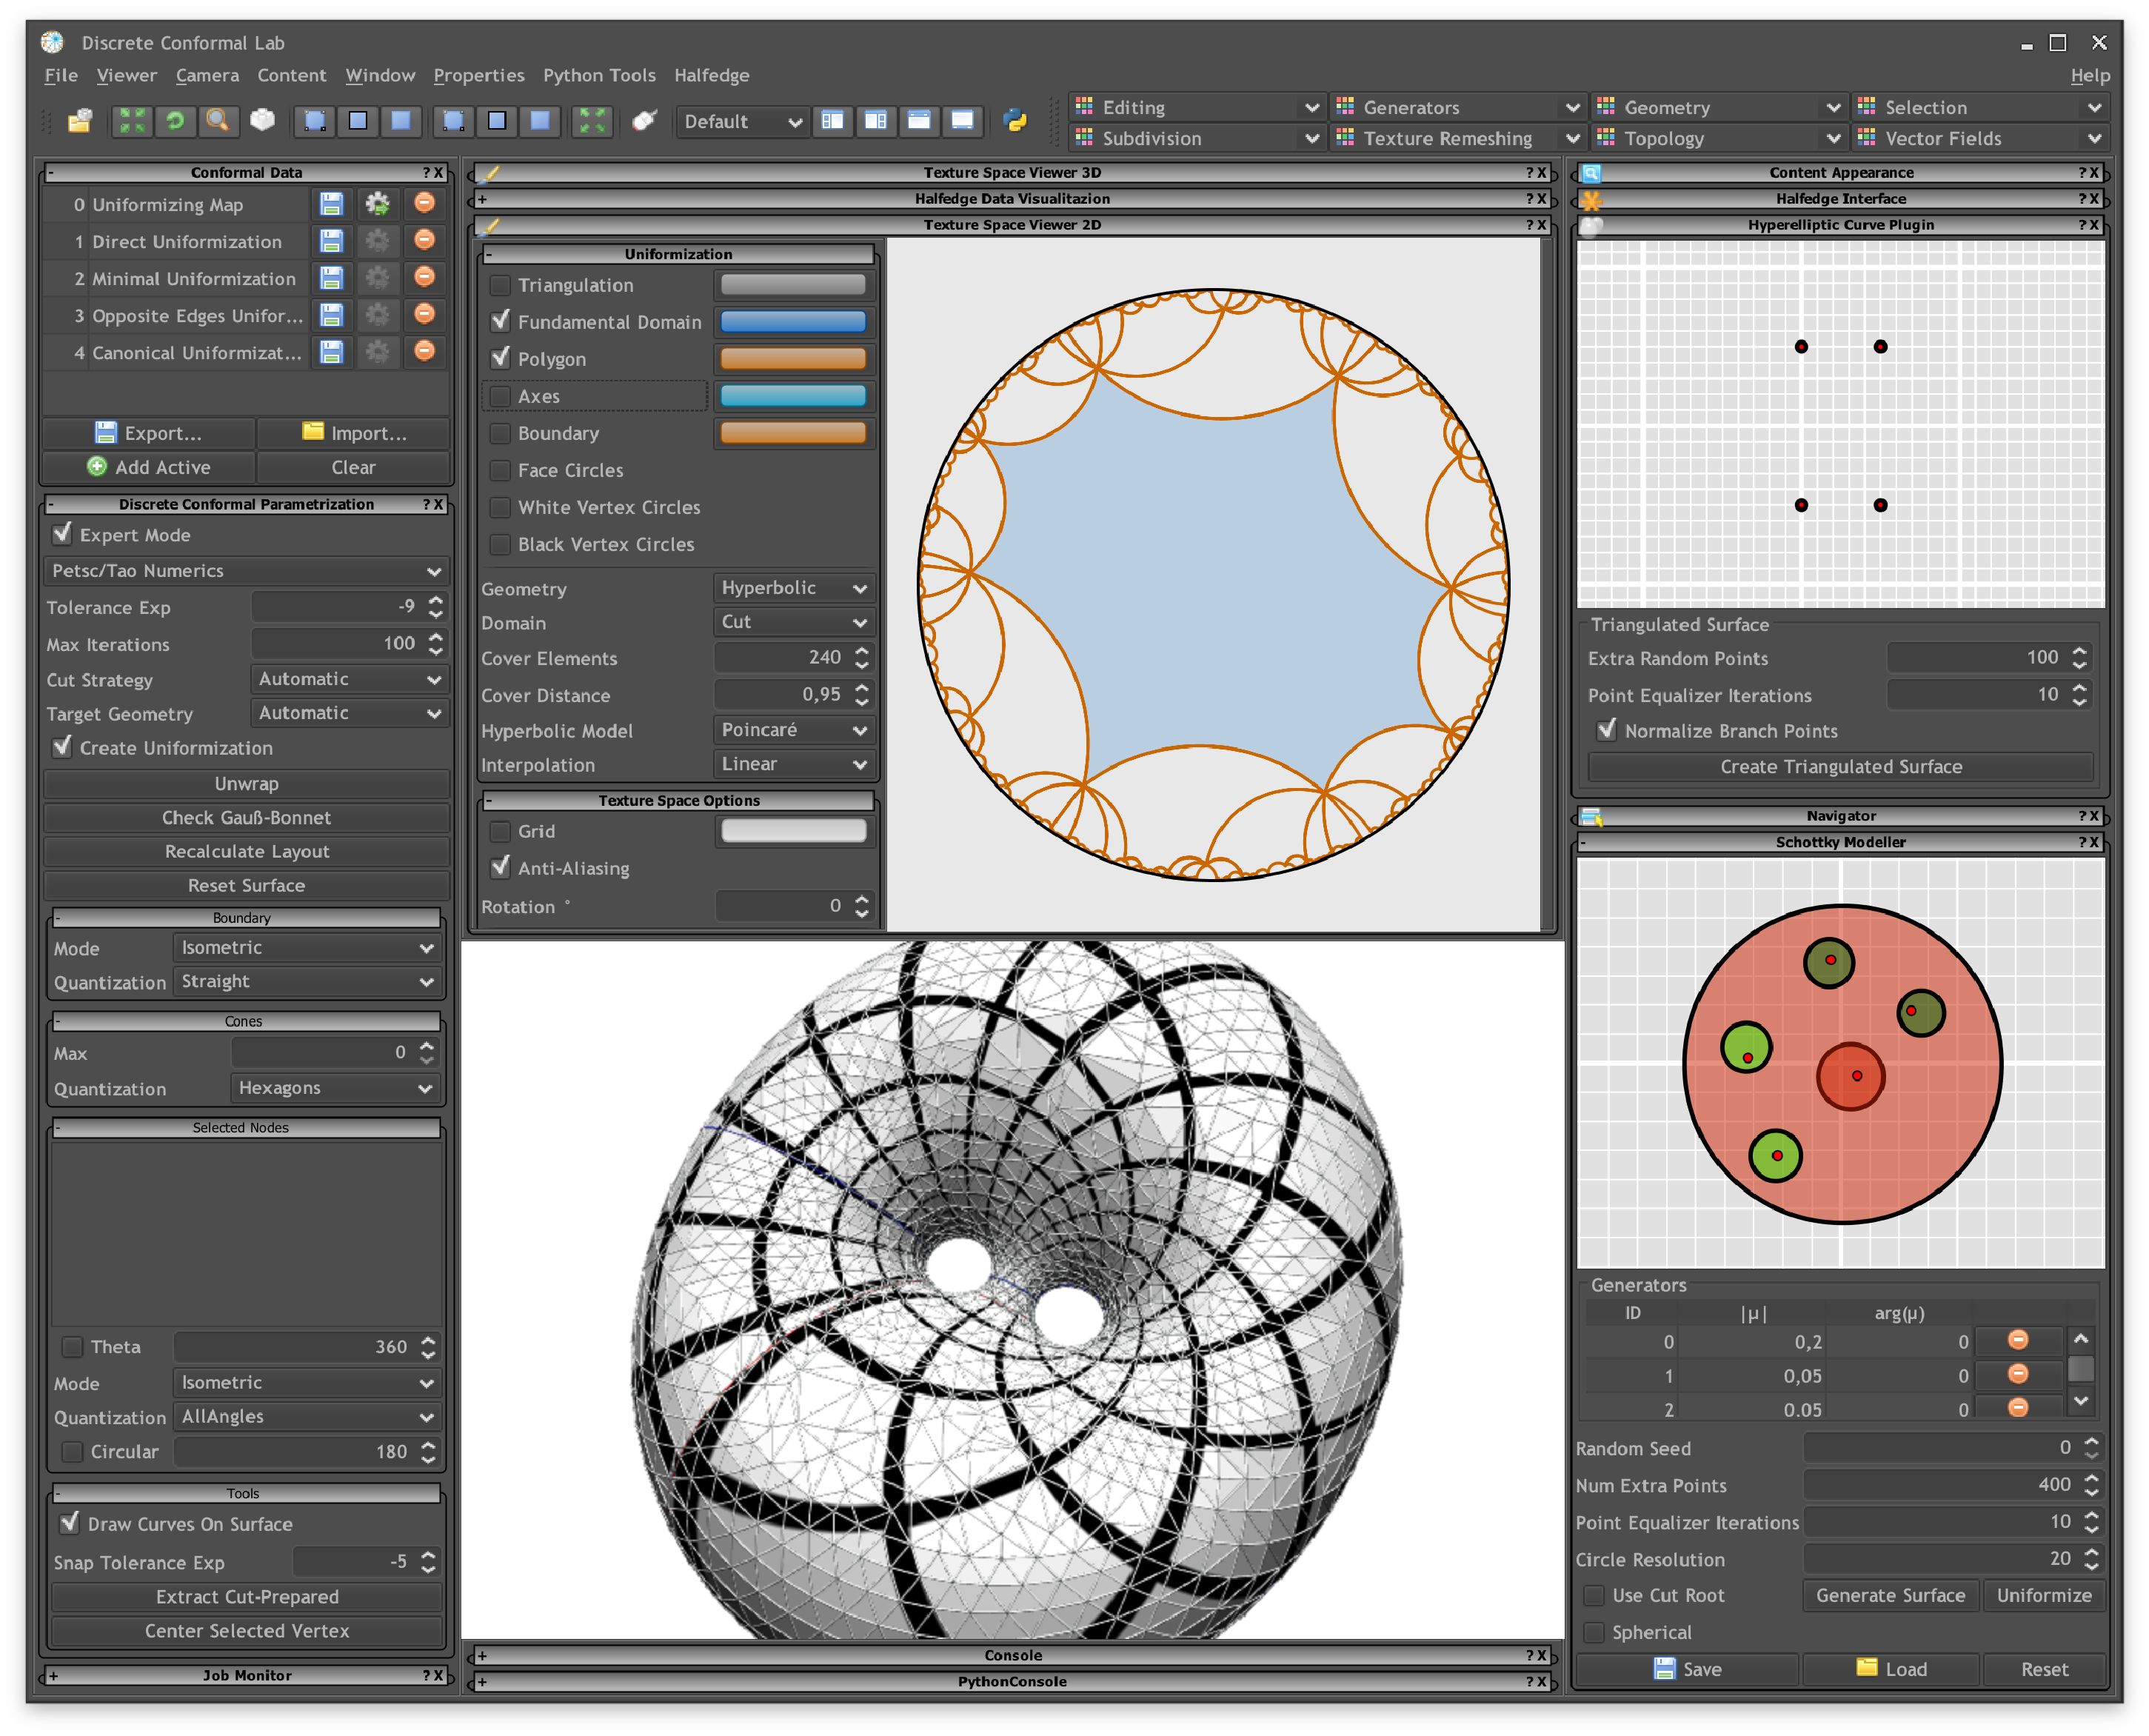
\includegraphics[width=1.0\linewidth]{conformllab/conformallab.pdf}
\caption{The user interface window of {\sc ConformalLab}.}
\label{fig:conformal_window}
\end{figure}

This chapter enables the reader to reproduce examples contained in this work
that involve discrete uniformization of Riemann surfaces, see
Chapter~\ref{chp:uniformization}, and applications of conformal mappings of
Part~\ref{part:applications}. The author has written {\sc Java} software, {\sc
ConformalLab}, to calculate the corresponding data.  The software and the data
is included on the accompanying CD, see also Section~\ref{chp:cd_content}. 

{\sc ConformalLab} is designed to be used via a graphical user interface, see
Figure~\ref{fig:conformal_window}. To store resulting data an XML format is
used. We describe this format in Section~\ref{sec:conformal_data}. The
graphical user interface is described in Section~\ref{sec:conformallab_ui}.
{\sc ConformalLab} uses {\sc JRworkspace}, see Chapter~\ref{chp:jrworkspace},
to implement its user interface. This allows the user interface to be divided
into panels which serve separate purposes.  {\sc ConformalLab} uses {\sc
HalfEdge} and {\sc HalfEdgeTools}, see Chapter~\ref{chp:halfedge}, to work with
discrete surfaces.


\section{XML data format}
\label{sec:conformal_data}
To store and process data {\sc ConformalLab} uses an {\sc XML} data format.
All examples presented in Chapter~\ref{chp:uniformization} are stored in
this format.  All XML data is contained in the XML namespace {\tt
http://www.varylab.com/conformallab/types}.


{\bf Schottky data} 

A Riemann surface can be given by Schottky data, see Section~\ref{sec:schottky}. 
An example is shown in
Listing~\ref{lst:schottky_xml}. {\tt SchottkyData} can include one or more {\tt
SchottkyGenerator}s. A {\tt SchottkyGenerator} defines fix points $A$ and
$B$, the complex number $\mu$, and a {\tt Circle}. This circle is required to
contain $A$ and must not contain $B$. If there are more that one generator,
then the circles an their images must not intersect.

\begin{lstlisting}[label=lst:schottky_xml, caption={A torus given by Schottky data}, 
numbers=none, language=XML, captionpos=b]
<SchottkyData name="Schottky">
	<SchottkyGenerator>
		<A re="-1.0" im="0.0"/>
		<B re="1.0" im="0.0"/>
		<Mu re="0.25" im="0.0"/>
		<Circle radius="1.3">
			<Center re="-1.6" im="0.0"/>
		</Circle>
	</SchottkyGenerator>
</SchottkyData>
\end{lstlisting}

{\bf Hyperelliptic data} 

{\tt HyperEllipticAlgebraicCurve}s as used in the examples of
Section~\ref{sec:elliptic_curves} and \ref{sec:hyperelliptic} are
given by the location of their branch points in the complex plane. All points
must be distinct. Listing~\ref{lst:hyperelliptic_xml} shows the XML
representation of an elliptic algebraic curve defining a Riemann surface of
genus~$1$. The point at infinity cannot be specified and is implicitly given if
an odd number of branch points is listed.

\begin{lstlisting}[label=lst:hyperelliptic_xml, caption={A torus given as 
hyperelliptic data}, numbers=none, language=XML, captionpos=b]
<HyperEllipticAlgebraicCurve name="Curve g2">
	<BranchPoint re="-0.5" im="-1.0"/>
	<BranchPoint re="0.5" im="-1.0"/>
	<BranchPoint re="1.0" im="0.0"/>
	<BranchPoint re="-1.0" im="0.0"/>
</HyperEllipticAlgebraicCurve>
\end{lstlisting}

{\bf Fuchsian data}

A Riemann surface given by Fuchsian data ({\tt UniformizationData}) is
represented by generators of the corresponding Fuchsian group and their inverse
elements as elements of $PSL(2,\mathbb R)$ ({\tt UniformizingGroup} and {\tt
IsometryPSL2R} XML nodes). In addition to the group a fundamental polygon is
defined by its vertices and edges. In Listing~\ref{lst:fuchsian_xml} the
uniformizing group of euclidean motions defines the structure of a flat torus.
The {\tt FundamentalPolygon} is a parallelogram. There is only one {\tt
FundamentalVertex} since all vertices of the parallelogram are identified.
There are four {\tt FundamentalEdge}s each of which is identified with its
opposite edge of the parallelogram. Each {\tt FundamentalEdge} defines a {\tt
StartPosition} in $\mathbb C$ that is interpreted as an element of $\mathbb R
P^2$. The polygon is positively oriented.

\begin{lstlisting}[label=lst:fuchsian_xml, caption={A torus given by its Fuchsian uniformizing group and a corresponding fundamental polygon. The elements of the group are either euclidean motions or hyperbolic motions given as elements of $PSL(2, \mathbb R)$.}, numbers=none, language=XML, captionpos=b]
<UniformizationData name="Direct Uniformization">
	<UniformizingGroup>
		<IsometryPSL2R 
			m11="1.0" m12="0.0" m13="1.0" 
			m21="0.0" m22="1.0" m23="0.0" 
			m31="0.0" m32="0.0" m33="1.0"
		/>
		<IsometryPSL2R 
			m11="1.0" m12="0.0" m13="0.0" 
			m21="0.0" m22="1.0" m23="1.0" 
			m31="0.0" m32="0.0" m33="1.0"
		/>
		<IsometryPSL2R 
			m11="1.0" m12="0.0" m13="-1.0" 
			m21="0.0" m22="1.0" m23="0.0" 
			m31="0.0" m32="0.0" m33="1.0"
		/>
		<IsometryPSL2R 
			m11="1.0" m12="0.0" m13="0.0" 
			m21="0.0" m22="1.0" m23="-1.0" 
			m31="0.0" m32="0.0" m33="1.0"
		/>
	</UniformizingGroup>
	<FundamentalPolygon>
		<FundamentalVertex index="0"/>
		<FundamentalEdge index="0" nextEdge="1" previousEdge="3" identifiedEdge="2" startVertex="0">
			<StartPosition re="0.0" im="0.0"/>
		</FundamentalEdge>
		<FundamentalEdge index="1" nextEdge="2" previousEdge="0" identifiedEdge="3" startVertex="0">
			<StartPosition re="1.0" im="0.0"/>
		</FundamentalEdge>
		<FundamentalEdge index="2" nextEdge="3" previousEdge="1" identifiedEdge="0" startVertex="0">
			<StartPosition re="1.0" im="1.0"/>
		</FundamentalEdge>
		<FundamentalEdge index="3" nextEdge="0" previousEdge="2" identifiedEdge="1" startVertex="0">
			<StartPosition re="0.0" im="1.0"/>
		</FundamentalEdge>
	</FundamentalPolygon>
</UniformizationData>
\end{lstlisting}

{\bf Discrete data} 

To specify discrete data we use the concept of half edge data structure, see
also Chapter~\ref{chp:halfedge}. Listing~\ref{lst:halfedge_xml} shows the
structure of a {\tt HalfedgeEmbedding}. {\tt Vertices} are assigned coordinates
in $\mathbb RP^3$ and their index. {\tt Halfedge} nodes specify indices of
incident faces, edges, and vertices as defined in Section~\ref{sec:halfedge}.
In addition the data needed to specify the combinatorics of the halfedge
data structure one can specify identifications of vertices and edges. An {\tt
Identification} node contains all vertices that are identified. Consider a
parallelogram fundamental domain of a flat torus. In the parallelogram all four
vertices are identified to form the topological torus. Also the edges of the
parallelogram are identified. An {\tt EdgeIdentification} node defines the four
half edges that belong to the pair of half edges on the torus.

\begin{lstlisting}[label=lst:halfedge_xml, caption={A torus given as {\tt HalfedegeEmbedding}
with identified edge pairs and vertices.}, numbers=none, language=XML, captionpos=b]
<HalfedgeEmbedding name="Uniformizing Map_domain">
	<Vertex x="0.0" y="0.0" z="0.0" w="1.0" index="0"/>
	<Vertex x="1.0" y="0.0" z="0.0" w="1.0" index="1"/>
	<Vertex x="1.0" y="1.0" z="0.0" w="1.0" index="2"/>
	<Vertex x="0.0" y="1.0" z="0.0" w="1.0" index="3"/>
	<Identification>
		<Vertex>0</Vertex>
		<Vertex>1</Vertex>
		<Vertex>2</Vertex>
		<Vertex>3</Vertex>
	</Identification>
	<Halfedge left="0" target="1" next="1" opposite="4" index="0"/>
	<Halfedge left="0" target="2" next="2" opposite="5" index="1"/>
	<Halfedge left="0" target="3" next="3" opposite="6" index="2"/>
	<Halfedge left="0" target="0" next="0" opposite="7" index="3"/>
	<Halfedge left="-1" target="0" next="7" opposite="0" index="4"/>
	<Halfedge left="-1" target="1" next="4" opposite="1" index="5"/>
	<Halfedge left="-1" target="2" next="5" opposite="2" index="6"/>
	<Halfedge left="-1" target="3" next="6" opposite="3" index="7"/>
	<EdgeIdentification edge1="0" edge2="4" edge3="2" edge4="6"/>
	<EdgeIdentification edge1="1" edge2="5" edge3="3" edge4="7"/>
	<Face index="0"/>
</HalfedgeEmbedding>
\end{lstlisting}

The {\tt HalfedgeEmbedding} data type can be used to define discrete maps
between discrete embeddings. A discrete map consists of a domain {\tt
HalfedgeEmbedding} and the corresponding image. Both nodes must define the same
number of vertices. The map is defined via vertex indices. A vertex $i$ from
the domain is mapped to the vertex with index $i$ in the image data structure,
see Listing~\ref{lst:halfedgemap_xml}.

\begin{lstlisting}[label=lst:halfedgemap_xml, caption={A discrete map is given by a pair of {\tt HalfedgeEmbedding}s, the {\tt Domain} and {\tt Image} of the map. Both are of type {\tt HalfedgeEmbedding}.}, numbers=none, language=XML, captionpos=b]
<HalfedgeMap name="Uniformizing Map">
	<Domain name="Uniformizing Map_domain">
		...
	</Domain>
	<Image name="Uniformizing Map_image">
		...
	</Image>
</HalfedgeMap>
\end{lstlisting}

A way of defining a discrete Riemann surface is to specify its discrete metric.
A {\tt DiscreteMetric} defines non-oriented {\tt MetricEdges} and their
lengths. {\tt MetricTriangles} are glues along those edges. All triangles are
oriented by the order of edges defined by attributes {\tt edge1}, {\tt edge2},
and {\tt edge3} respectively. By that we can only encode oriented discrete
Riemann surfaces using a {\tt DiscreteMetric}.  A simple example featuring a
Wente torus is shows in Listing~\ref{lst:discretemetric_xml}.

\begin{lstlisting}[label=lst:discretemetric_xml, caption={
A Wente torus given by a discrete metric. Vertices are given implicitly by following the order of triangle glueing.}, numbers=none, language=XML, captionpos=b]
<DiscreteMetric name="Wente Torus">
	<MetricEdge length="1.0" index="0"/>
	<MetricEdge length="1.0" index="1"/>
	<MetricEdge length="1.0" index="2"/>
	<MetricTriangle edge1="0" edge2="1" edge3="2"/>
	<MetricTriangle edge1="0" edge2="1" edge3="2"/>
</DiscreteMetric>
\end{lstlisting}

{\bf Data lists}

Each of the data nodes as described above can appear in an element of type {\tt
ConformalDataList}. A typical XML file representing the data of an example of
Chapter~\ref{chp:uniformization} contains input data, e.g. {\tt
SchottkyData} and {\tt DiscreteMetric}, as well as the resulting output
embedding and uniformization data represented as {\tt HalfedgeEmbedding} and
{\tt UniformizationData}.

\begin{lstlisting}[label=lst:datalist_xml, caption={A list of data XML nodes as the result of an algorithm calculating the Fuchsian uniformization of a genus $1$ Riemann surface given by Schottky data.}, numbers=none, language=XML, captionpos=b]
<ConformalDataList>
	<SchottkyData name="Schottky Data g1">
		...
	</SchottkyData>
	<DiscreteMetric name="Input Schottky Data Metric">
		...
	</DiscreteMetric>
	<HalfedgeEmbedding name="Output Euclidean Embedding">
		...
	</HalfedgeEmbedding>
	<HalfedgeMap name="Uniformizing Map">
		<Domain name="Uniformizing Map_domain">
			...
		</Domain>
		<Image name="Uniformizing Map_image">
			...
		</Image>
	</HalfedgeMap>
	<UniformizationData name="Direct Uniformization">
		...
	</UniformizationData>
	<UniformizationData name="Minimal Uniformization">
		...
	</UniformizationData>
</ConformalDataList>
\end{lstlisting}

\section{Uniformization and conformal mappings} \label{sec:conformallab_ui} The
user interface of {\sc ConformalLab} is divided into panels which serve
separate purposes in the workflow of performing experiments with discrete
Riemann surfaces and conformal mappings.


{\bf Data import and export}

\begin{figure}
\centering
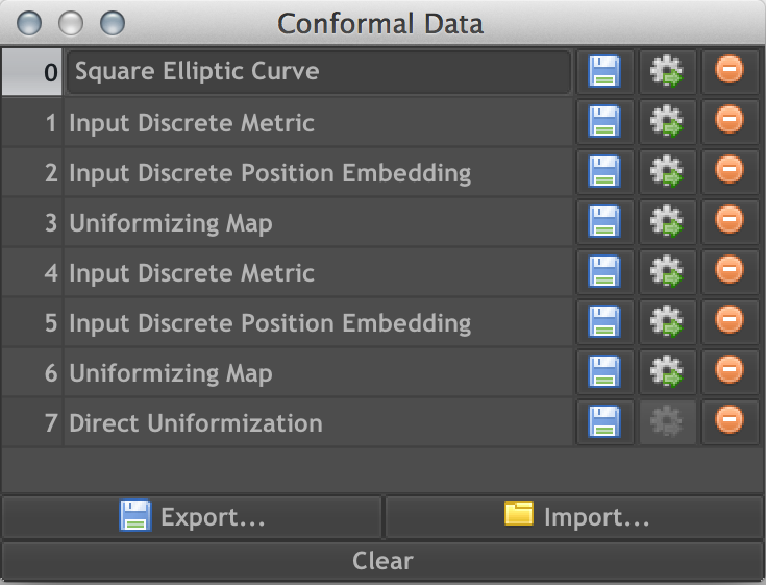
\includegraphics[width=0.35\linewidth]{conformllab/conformal_data.pdf}
\caption{Data import and export interface works with XML data files as described in 
Section~\ref{sec:conformal_data}.}
\label{fig:data_interface}
\end{figure}

The data import and export panel, see Figure~\ref{fig:data_interface}, provides functions to import and export XML data as described in Section~\ref{sec:conformal_data}.  
Data files can be loaded into memory via the Import button. A table lists the entries of the loaded file.  
Loadable are {\tt ConformalDataList} as well as single data instances. 
The entries of a {\tt ConformalDataList} are listed in the table of the panel. 

Each of the rows contains buttons to save the data to disk (blue disk), load it into the program (gear with green arrow), or delete it from the list (red circle).  
The function of the load button depends on the data type. 
A {\tt HalfedgeEmbedding} is loaded as geometry and is displayed in the 3D viewer. 
A {\tt HalfedgeMap} defines geometry together with texture coordinates and boundary identifications. 
If suitable boundary identification is given a uniformizing group is calculated and visualized. 
{\tt HyperEllipticAlgebraicCurve}s are loaded into the hyperelliptic curve panel of the user interface, see Figure~\ref{fig:conformal_main_generators}, right-top.  
{\tt SchottkyData} is loaded into the Schottky modeler panel, see Figure~\ref{fig:conformal_main_generators}, right-bottom.


{\bf Hyperelliptic curves}

The hyperelliptic curve panel (Figure~\ref{fig:conformal_main_generators} right-top) is used to create branched triangulations of the doubly covered sphere.
Hyperelliptic curves are defined vie their branch points, see Section~\ref{sec:hyperelliptic} of Chapter~\ref{chp:uniformization}.
The user can add branch points by double-clicking in the graph paper view.
Double-clicking an existing point brings up a coordinate editor. 
The lower section of the panel defines parameters of mesh creation. 
The user can choose to add extra equally distributed random points to the triangulation.
These points can be further optimized to form a more regular triangulation.
The number of point equalizer iterations defines the number of gradient decent steps in the optimization of the functional defined in Section~\ref{sec:spherical_triangulations}.
The location of the branch points can be normalized via a M{\"o}bius transformation on the sphere such that the center of mass of the points is the center of the sphere. For the details see Section~\ref{sec:moebius_normalization}.

\begin{figure}
\centering
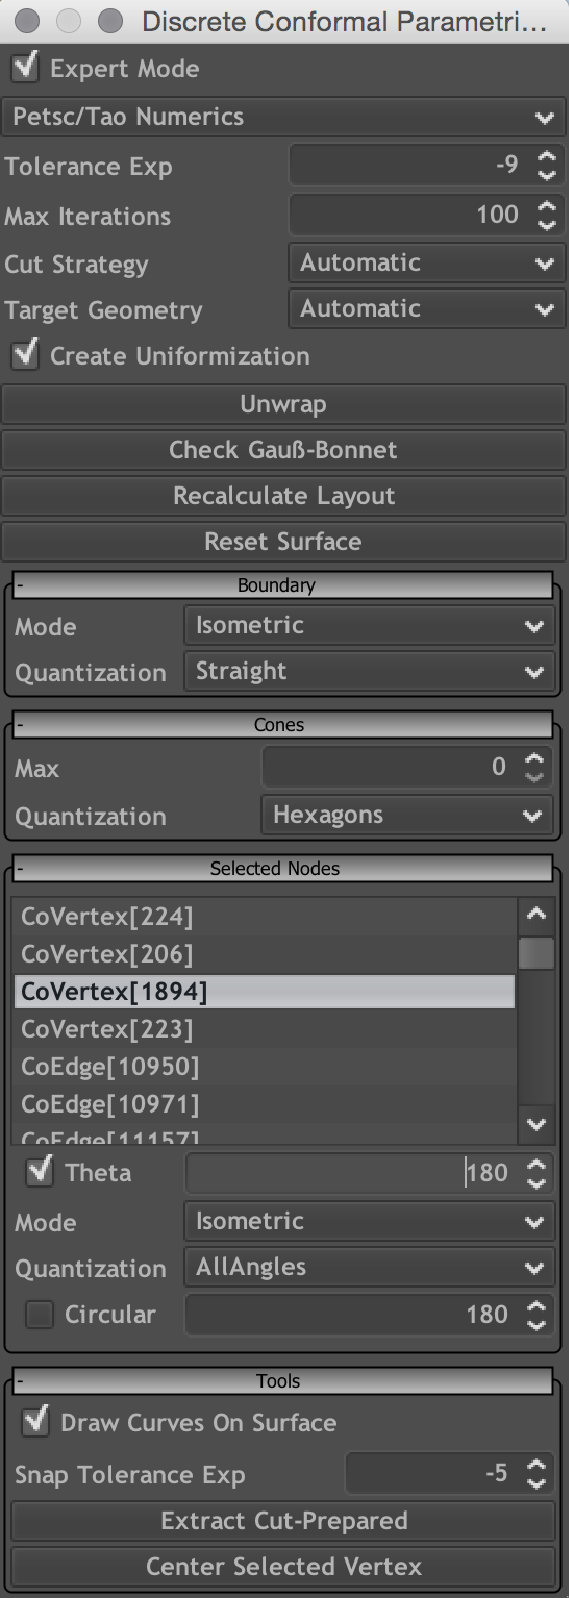
\includegraphics[width=0.45\linewidth]{conformllab/main_interface.pdf}\hfill
\begin{minipage}[b]{0.5\linewidth}
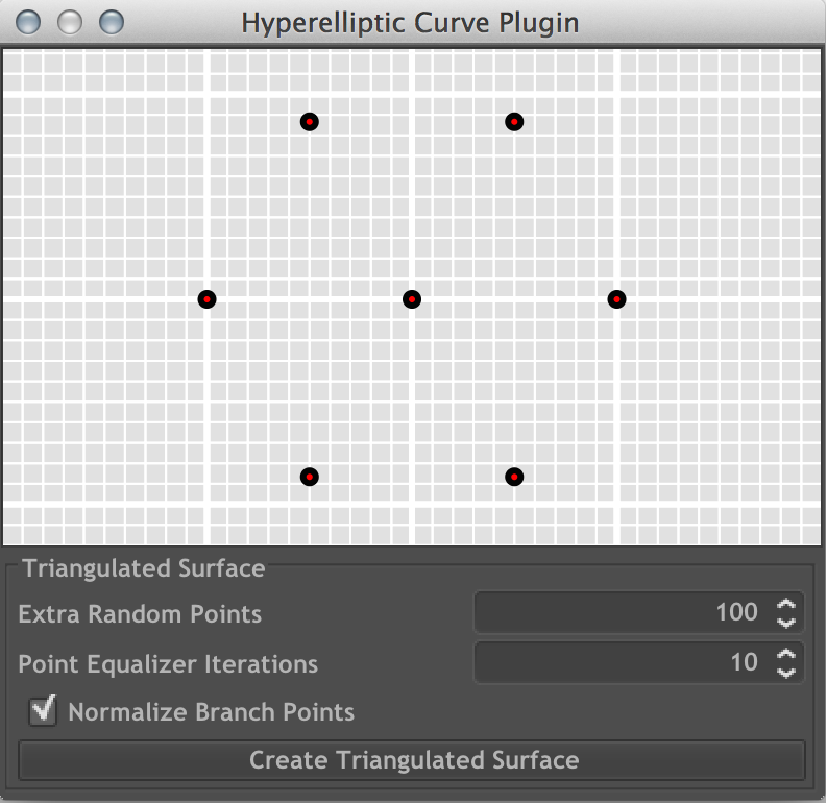
\includegraphics[width=\linewidth]{conformllab/hyperelliptic_curve.pdf}\\
\vskip 0.1cm
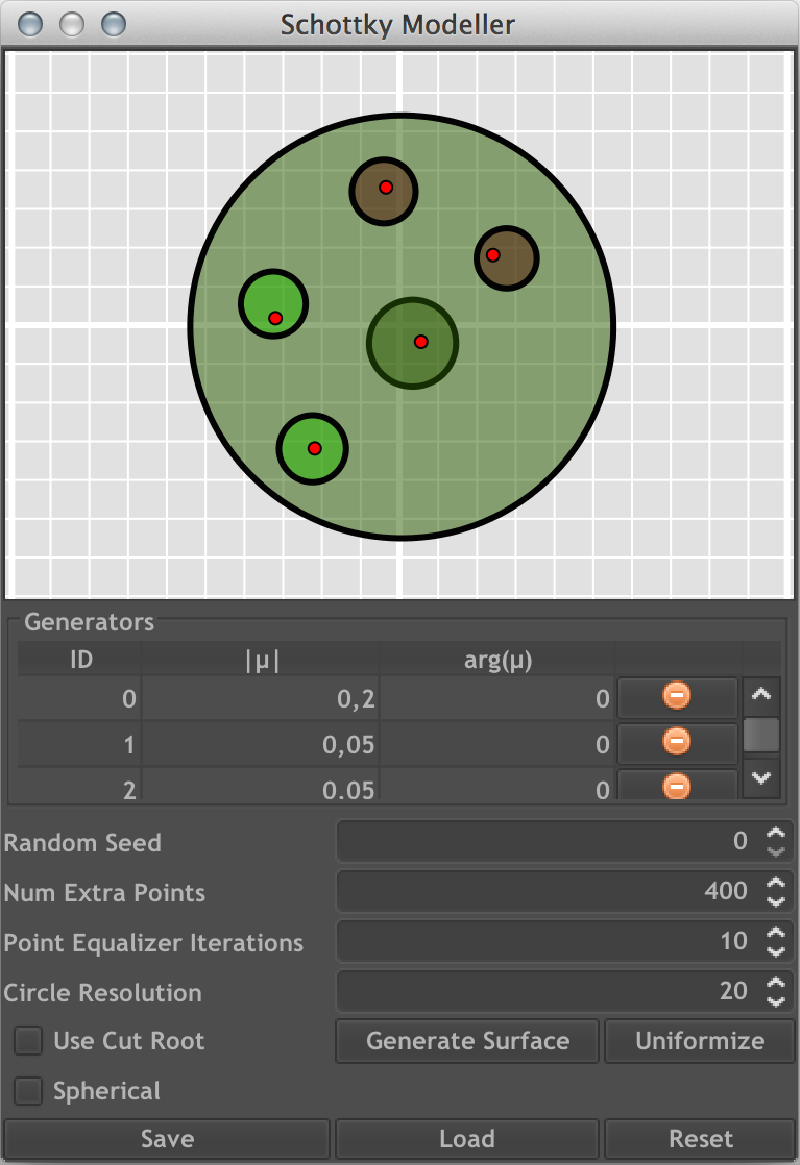
\includegraphics[width=\linewidth]{conformllab/schottky_modeller.pdf}
\end{minipage}
\caption{The main interface of {\sc ConformalLab} (left). Hyperelliptic curve interface (right-top).
Schottky modeler user interface (right-bottom).}
\label{fig:conformal_main_generators}
\end{figure}

{\bf Schottky modeler}

The Schottky modeler panel (See Figure~\ref{fig:conformal_main_generators} right-bottom) generates Schottky data for Riemann surfaces, see Section~\ref{sec:schottky}. 

In the graph-paper view the circles and fix points of the generators are shown and can be modified. 
Moving a fix point of a generator transforms the corresponding circle as the image of the circle around the other fix point. 
Moving a circle causes the image circle to be recalculated. 
New generators can be added from the right-click menu. 
The parameter $\mu$ of each generator can be edited in the table below.
Similar to the generation of hyperelliptic data additional points can be added and modified my a regularization process. 
In addition to this the number of points that discretize the circles can be given.

The \emph{Generate Surface} button creates a triangulated surface together with a metric calculated from the Schottky data. 
This surface can then be uniformized via the main interface. 
The \emph{Uniformize} button directly creates a uniformization and introduces cuts along the circles of the Schottky data. 
The corresponding fundamental domain is then bounded by the pre-images of the circles and curves connecting them.
The examples of Section~\ref{sec:schottky} use this fundamental domain.

{\bf Main interface}

The main interface of {\sc ConformalLab} offers all functions to create the conformal mapping examples described in this work (see Figure~\ref{fig:conformal_main_generators} left). 
It is divided into sections that we cover briefly from top to bottom. 

The user interface comes in two modi, normal mode and expert mode, that can be switched with the \emph{Expert Mode} check box. 
In normal mode we show only user interface elements that are needed by users of {\sc VaryLab}.
It supports basic surface parameterization and remeshing of discrete surfaces, see Chapter~\ref{chp:varylab}. 
All other elements are hidden in normal mode.

{\sc ConformalLab} uses two numerical libraries to implement energy minimization. 
They can be chosen from the drop-down box at the top of the panel. 
\emph{Petsc/Tao Numerics} selects the {\sc PETSc/TAO} C++ library, see~\cite{petsc-web-page, tao-user-ref}. 
We use the Newton Trust Region (NTR) method as implemented by {\sc PETSc/TAO} whenever we have calculated the Hessian matrix for the corresponding energy. 
Otherwise we use LMVM method with default configuration. 
\emph{Java/MTJ Numerics} implements a version of Newtons method using the linear algebra package MTJ, see~\cite{mtj-website}. 
We implement a backtracking line search as described in~\cite[pp.~464]{boyd2004convex}.

The \emph{Tolerance Exp} and \emph{Max Iterations} options are used during energy minimization. 
Tolerance means absolute tolerance as defined by {\sc PETSc/TAO}. 
The minimizer converges if the Frobenius norm of the gradient is less than ten to the selected exponent. The \emph{Max Iterations} value means the maximum number of Newton steps carried out by the optimization library.

For surfaces with genus one or higher a \emph{Cut Strategy} can be chosen from a drop down menu. 
\emph{Automatic} creates cuts along precomputed edge cycles such that the resulting surface is simply connected. 
At the same time the number of edges that have been cut is small. 
\emph{Selection} uses user selected edges as cutting cycles. 
This is primarily used to create manual cutting curves. 
\emph{NoCuts} does not cut the mesh. 
This is needed, e.g., in the workflow of creating periodic maps as described in Chapter~\ref{chp:periodic_conformal_maps}.

The \emph{Target Geometry} defines the geometry for the domain of parameterization. 
A value of "Automatic" selects spherical geometry for surfaces of genus zero, euclidean geometry for genus one, and hyperbolic geometry for surfaces of higher genus.

The \emph{Create Uniformization} check box defines whether a uniformization is calculated when pressing the \emph{Unwrap} button. 
The program manages two instances of the surface: The input surface and the "unwrapped" surface. Pressing the \emph{Reset} button reloads the input surface.

To check boundary conditions and internal cone angles pressing \emph{Check Gau\ss-Bonnet} prints the integrals over boundary curvature and Gaussian curvature to the console. 
\[\sum_{v \in \partial S} \left(\pi - \theta_v\right) + \sum_{v \in \mathring{S}}\left(2\pi - \theta_v\right)\]
By default all interior angles are set to $2\pi$ unless otherwise defined by manual settings in the \emph{Selected Nodes} section. The angle at a boundary vertex is defined either manually or calculated via settings in the \emph{Boundary} section.

The \emph{Boundary} section contains the settings that define boundary conditions at vertices of the mesh. 
The default mode is \emph{Isometric}. In this mode boundary edges on the surface and in texture space have the same length. If boundary angles on the surface are not far away from desired angles in the domain then \emph{Quantized Angles} mode can be used to define boundary angles via angles on the surface and a quantization function selected from the \emph{Quantization} drop down:

\begin{eqnarray*}
	Q_{\mathrm{AllAngles}}(\theta) &=& \theta \\
	Q_{\mathrm{Quads}}(\theta) &=& \mathrm{round}\left(\theta, \frac{\pi}{4}\right) \\
	Q_{\mathrm{QuadsStrict}}(\theta) &=& \mathrm{round}\left(\theta, \frac{\pi}{2}\right) \\
	Q_{\mathrm{Hexagons}}(\theta) &=& \mathrm{round}\left(\theta, \frac{\pi}{3}\right) \\
	Q_{\mathrm{Triangles}}(\theta) &=& \mathrm{round}\left(\theta, \frac{\pi}{6}\right).
\end{eqnarray*}

Here $\mathrm{round(x,y)}$ maps $x$ to the nearest multiple of $y$.
\emph{Conformal Curvature} boundary mode defines angles via a vector field on boundary edges as described in Chapter~\ref{chp:quasiisothermic}. 
The \emph{Circle} option creates a map to the unit circle. 
Using this option we invoke the method described in Sections~\ref{sec:riemann_map} and~\ref{sec:circle_domains}. 
In \emph{Read Isometric Angles} mode the program performs conformal parameterization with isometric boundary. 
Additionally resulting boundary angles are read into manual boundary conditions for later usage, e.g., with \emph{QuantizedAnglePeriods} boundary conditions, that modifies boundary angles as described in Section~\ref{sec:boundary}.

The \emph{Cones} section lets you specify automatically placed cones as introduced by~\cite{Springborn2008}. You can prescribe the number and quantization function as defined above.

Manual boundary conditions can be specified in the \emph{Selected Nodes} section. 
Here the currently selected vertices and edges are listed. 
Selected vertices can have manually prescribed angles~$\theta$ or boundary modes as described above. 
Edges can be set circular with a certain intersection angle of circum-circles, see Section~\ref{sec:riemann_map} or Section~\ref{sec:circle_domains}. 
The default angle is $180\degree$, i.e., the two adjacent triangles form a circular quadrilateral.

The \emph{Tools} section include commands that operate on a readily computed uniformization of a surface of higher genus $g\geq 2$. 
The \emph{Draw Curves On Surface} check box calculates, if activated, images of the edges of fundamental domains. 
These curves are displayed on the surface, see, e.g., Figure~\ref{fig:lawson_embedding} left. 
The \emph{Extract Cut-Prepared} button creates a new surface as a copy of the current input data including edges of a fundamental polygon. 
You can use this to create uniformized surfaces where the triangulation fits perfectly into the fundamental polygon. 
The \emph{Center Selected Vertex} button applies a hyperbolic motion to the texture coordinates such that the selected vertex becomes the center of the unit disk.

{\bf Visualization}

\begin{figure}
\resizebox{\textwidth}{!}{
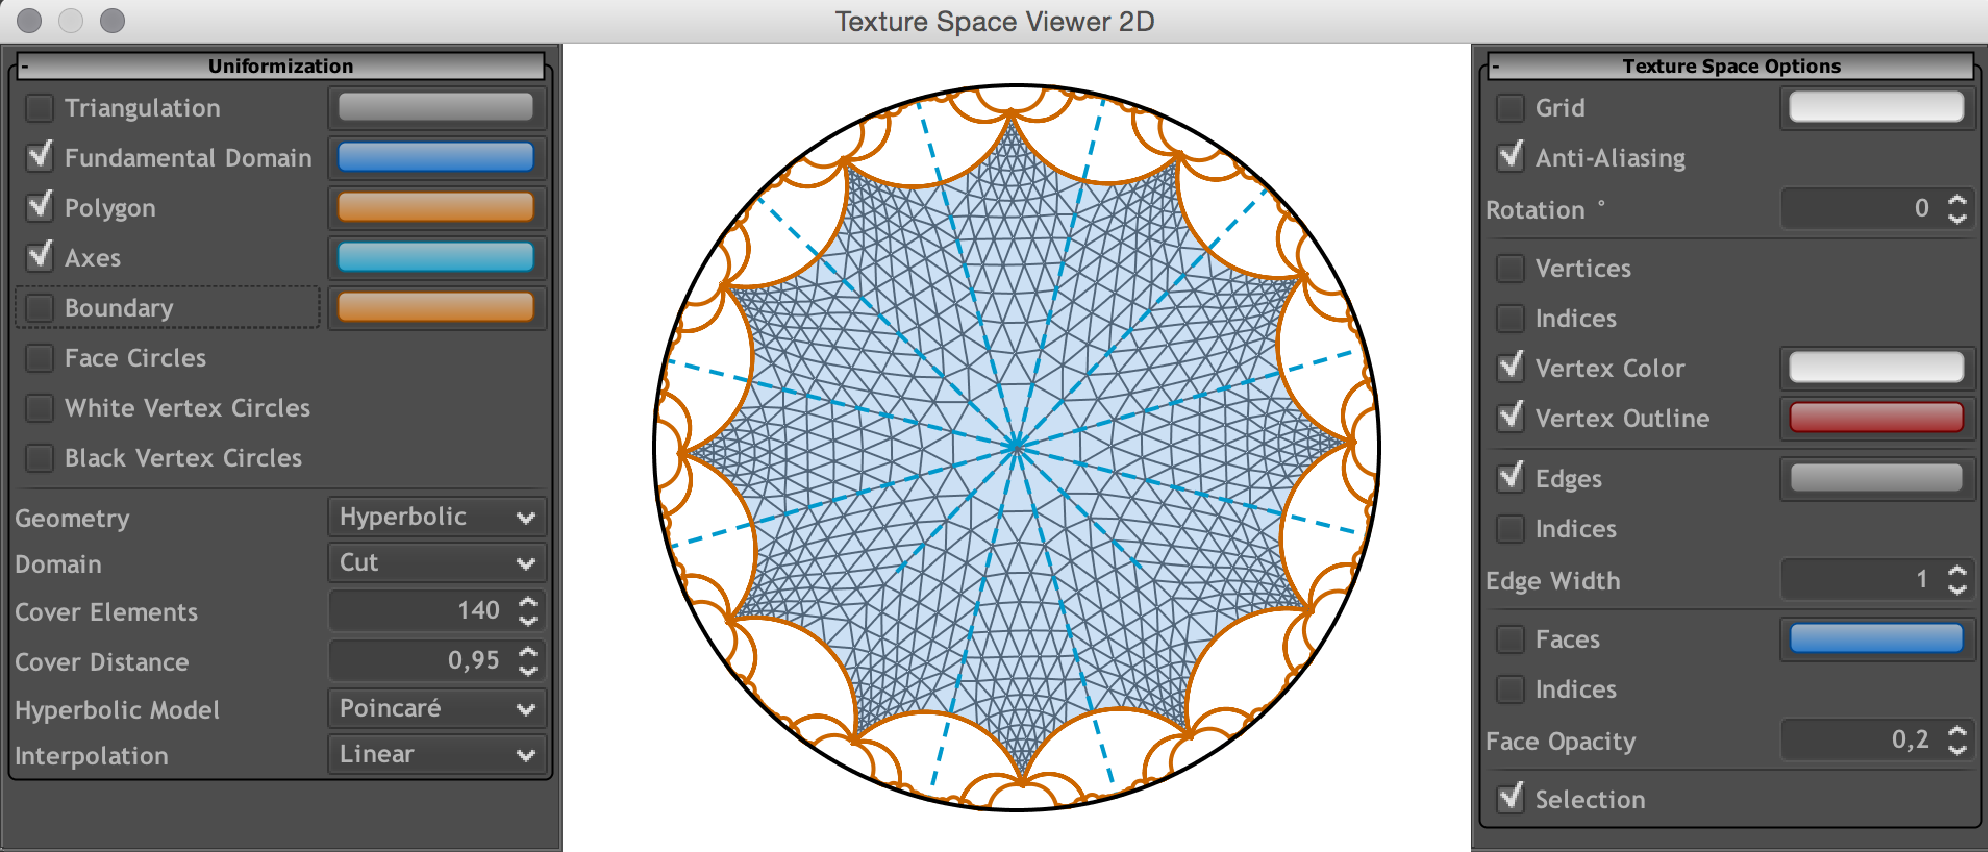
\includegraphics[width=0.7\linewidth]{conformllab/visualization.pdf}
}
\caption{Visualization interface. It shows the domain of parameterization for euclidean and hyperbolic geometry. 
For hyperbolic images the Klein model, Poinar\'e disk model, and the half-plane model are supported.}
\label{fig:visualization_interfaces}
\end{figure}

The \emph{Visualization Interface}, see Figure~\ref{fig:visualization_interfaces}, shows the domain of uniformization. 
Additionally depending on the geometry one can visualize extra structures like fundamental polygons, universal cover, or identification maps. 
It is divided into two sections. The generic \emph{Texture Space Options} define options for the mapping of the mesh. 

The \emph{Uniformization} section defines the visualization of the current uniformization. 
\emph{Triangulation} activates the visualization of the mesh across the universal cover of the surface using as many group elements as specifies in the \emph{Cover Elements} and \emph{Cover Distance} input fields. 
The fundamental polygon corresponding to the identity group element can be visualized with the \emph{Fundamental Domain} check box. Its axes of identification can be shown with the \emph{Axes} check box. 
The \emph{Polygon} box enables the visualization of polygon edges for all group elements defined by \emph{Cover Elements} and \emph{Cover Distance}. 
If the triangulation exhibits a circle pattern face circles through vertices of faces can be shown.

The \emph{Geometry} option is set automatically during calculation of uniformization but can be adjusted from the check box. The automatic value depends on the genus of the surface alone and may not be the correct choice. The program calculates four different fundamental domains that can be selected from the \emph{Domain} drop down see Section~\ref{sec:polygons_generators}. If the selected geometry is \emph{Hyperbolic} you can choose the corresponding model. {\sc ConformalLab} supports visualization of \emph{Poicar\'e}, \emph{Klein}, and \emph{HalfPlane} model.

The \emph{Interpolation} option lets you select how textures are interpolated on the current model. 
%see Section~\ref{chp:projective_interpolation}. 
If a texture image is active the 3D visualization is updated accordingly.


\subfilebibliography
\end{document}

%%% Local Variables:
%%% TeX-master: "Thesis.tex"
%%% End:
